% % % % % % % % % % % % % % % % % % % % % % % % % % % % % % % % % % % % % % % % % % % %
%                                                                                     %
% Short Sectioned Assignment LaTeX Template Version 1.0 (5/5/12)                      %
% This template has been downloaded from: http://www.LaTeXTemplates.com               %
%                                                                                     %
% Original author:  Frits Wenneker (http://www.howtotex.com)                          %
%                                                                                     %
% Modified by: Fco Javier Sueza Rodríguez (fcosueza@disroot.org)                      %
%                                                                                     %
% Changes:                                                                            %
%	    - Custom Chapters, Sections and Subsections (titlesec package)                %
%           - Document type scrbook (oneside)                                         %
%           - Use babel-lang-spanish package and marvosym                             %
%           - Use hyperref, enumitem, tcolorbox and glossaries packages               %
%           - Use Time New Roman (mathptmx), Helvetic and Courier fonts               %
%                                                                                     %
% License: CC BY-NC-SA 3.0 (http://creativecommons.org/licenses/by-nc-sa/3.0/)        %
%                                                                                     %
% % % % % % % % % % % % % % % % % % % % % % % % % % % % % % % % % % % % % % % % % % % %

%-----------------------------------------------%
%	              Packages                  %
%-----------------------------------------------%

\documentclass[paper=a4, fontsize=11pt, oneside]{scrbook}

% ---- Text Input/Output ----- %

\usepackage[T1]{fontenc}
\usepackage[utf8]{inputenc}
\usepackage{mathptmx}
\usepackage[scaled=.92]{helvet}
\usepackage{courier}
\usepackage[indent=12pt]{parskip}

\usepackage{geometry}
\geometry{verbose,tmargin=3cm,bmargin=3cm,lmargin=2.6cm,rmargin=2.6cm}

% ---- Language ----- %

\usepackage[spanish]{babel}
\usepackage{marvosym}

% ---- Another packages ---- %

\usepackage{amsmath,amsfonts,amsthm}
\usepackage{graphics,graphicx}
\usepackage{titlesec}
\usepackage{fancyhdr}
\usepackage{tcolorbox}
\usepackage{hyperref}
\usepackage{enumitem}
\usepackage[automake]{glossaries}

%--------------------------------------------------------------------%
%                      Customizing Document                          %
%--------------------------------------------------------------------%


% ----------- Custom Chapters, Sections and Subsections -------------- %

\titleformat{\chapter}[display]
			{\bfseries\Huge}
			{Tema \ \thechapter} {0.5ex}
			{\vspace{1ex}\centering}

\titleformat{\section}[hang]
			{\bfseries\Large}
			{\thesection}{0.5em}{}

\titleformat{\subsection}[hang]
			{\bfseries\large}
			{\thesubsection}{0.5em}{}

\titleformat{\subsubsection}[hang]
			{\bfseries\large}
			{\thesubsubsection}{0.5em}{}

\hypersetup{
    colorlinks=true,
    linkcolor=black,
    urlcolor=magenta
}

% ------------------- Custom heaaders and footers ------------------- %

\pagestyle{fancyplain}

\fancyhead[]{}
\fancyfoot[L]{}
\fancyfoot[C]{}
\fancyfoot[R]{\thepage}

\renewcommand{\headrulewidth}{0pt} % Remove header underlines
\renewcommand{\footrulewidth}{0pt} % Remove footer underlines

\setlength{\headheight}{13.6pt} % Customize the height of the header

% --------- Numbering equations, figures and tables ----------------- %

\numberwithin{equation}{section} % Number equations within sections
\numberwithin{figure}{section} % Number figures within sections
\numberwithin{table}{section} % Number tables within sections

% ------------------------ New Commands ----------------------------- %

\newcommand{\horrule}[1]{\rule{\linewidth}{#1}} % Create horizontal rule command


%----------------------------------------------------------------------------------------
%	TÍTULO Y DATOS DEL ALUMNO
%----------------------------------------------------------------------------------------

\title{
\vspace{10ex}
\normalfont \normalsize
\huge \textbf{Actividades de la Unidad 2}
}
\author{Francisco Javier Sueza Rodríguez}
\date{\normalsize\today}

%----------------------------------------------------------------------------------------
%                                     DOCUMENTO
%----------------------------------------------------------------------------------------
\begin{document}

\maketitle

\thispagestyle{empty}

\vspace{75ex}

\begin{center}
    \begin{tabular}{l l}
        \textbf{Centro}: & IES Aguadulce \\
        \textbf{Ciclo Formativo}: & Desarrollo Aplicaciones Web (Distancia)\\
        \textbf{Asignatura}: & Formación y Orientación Laboral\\
        \textbf{Tema}: & Tema 2 -  La Relación Colectiva en el Trabajo\\
    \end{tabular}
\end{center}

\newpage

\section{Actividad 1}
\subsection{Enunciado}
Seguro que has oído hablar del teletrabajo o estás trabajando así. Te invitamos a una reflexión sobre las ventajas y desventajas desde el punto de vista del trabajador.

\subsection{Respuesta}
El \textbf{teletrabajo} es una modalidad de trabajo que, especialmente durante la pandemia, a aumentado considerablemente. Esta es una modalidad que tiene, desde mi punto de vista, bastante ventajas y alguno inconvenientes.

Respecto a las \textbf{ventajas}, el teletrabajo ayuda a la conciliación familiar, ya que el realizar el trabajo desde casa podemos pasar más tiempo con la familia, facilitando en los casos que sea necesario cuidar de algunos miembros de la familiar durante más tiempo. Además, según algunos estudios, el teletrabajo incrementa la productividad. Algo que tampoco sorprende, ya que ademas de trabajar en un ambiente familiar más distendido, se evitan desplazamientos, que a veces pueden generar estrés, especialmente en grandes ciudades con mucho tráfico en horas concretas.

Por otro lado, el teletrabajo tiene sus \textbf{desventajas}. Por un lado, no todos los puestos de trabajo son susceptibles de ejercer en esta modalidad, hay empleos que son necesariamente presenciales y que no pueden desarrollarse en la distancia, como cualquier empleo en hostelería, dependientes en negocios, trabajos de la construcción, etc. Además, dependiendo de las circunstancias de cada uno en su casa, puede que el ambiente no sea el más adecuado para desarrollar el trabajo, por ejemplo, porque no hay la suficiente tranquilidad para concentrarse. Un factor que tiene también en contra es que se reduce la socialización que si tendríamos acudiendo a la oficina. Aunque hagamos videoconferencias a diario, no es lo mismo que el trato cara a cara con los compañeros.

En definitiva, el teletrabajo tiene sus virtudes y sus defectos, y ya dependerá de cada persona y cada situación si es más o menos idóneo para el correcto desarrollo de las funciones propias del puesto de trabajo.

\section{Actividad 2}
\subsection{Enunciado}

\subsubsection*{La Negociación Colectiva}
Busca un convenio colectivo vigente aplicable al sector profesional de informática, que no esté además tratado o ejemplificado en el tema, y responde justificadamente a las siguientes cuestiones:

\begin{enumerate}
    \item Haz una captura legible en el que se identifique el convenio elegible y añade enlace activo al mismo para que pueda consultarlo.
    \item En cuanto al contenido mínimo del convenio mediante captura muestra el artículo que haga referencia a los siguientes apartado. Es necesario tras la captura copiar la \textbf{información pedida}:
    \begin{enumerate}
        \item Indicación de las partes que lo han negociado.
        \item Ámbito de aplicación personal, funcional, territorial y temporal
    \end{enumerate}
    \item Realiza una captura referente a la planificación anual de las vacaciones y copia debajo el texto.
    \item Busca un artículo del convenio que te llame la atención (por interés ,curiosidad, desacuerdo..etc) sobre algún tipo de contenido:
    \begin{enumerate}
        \item Explica qué tipo de contenido trata
        \item Haz una captura del mismo y copia debajo el artículo capturado.
        \item Justifica tu elección
    \end{enumerate}
\end{enumerate}

\subsection{Respuesta}

\begin{enumerate}
    \item Para esta actividad, se ha elegido el \textbf{XIX Convenio colectivo del sector de empresas de ingeniería y oficinas de estudios técnicos}, uno de los que se puede aplicar a los programadores de aplicaciones informáticas, el cuál se puede encontrar en la \href{https://www.boe.es/diario_boe/txt.php?id=BOE-A-2019-14977}{página del BOE} correspondiente.

    En la siguiente figura de muestra una imagen del encabezado del convenio colectivo.

    \begin{figure}[H]
        \centering
        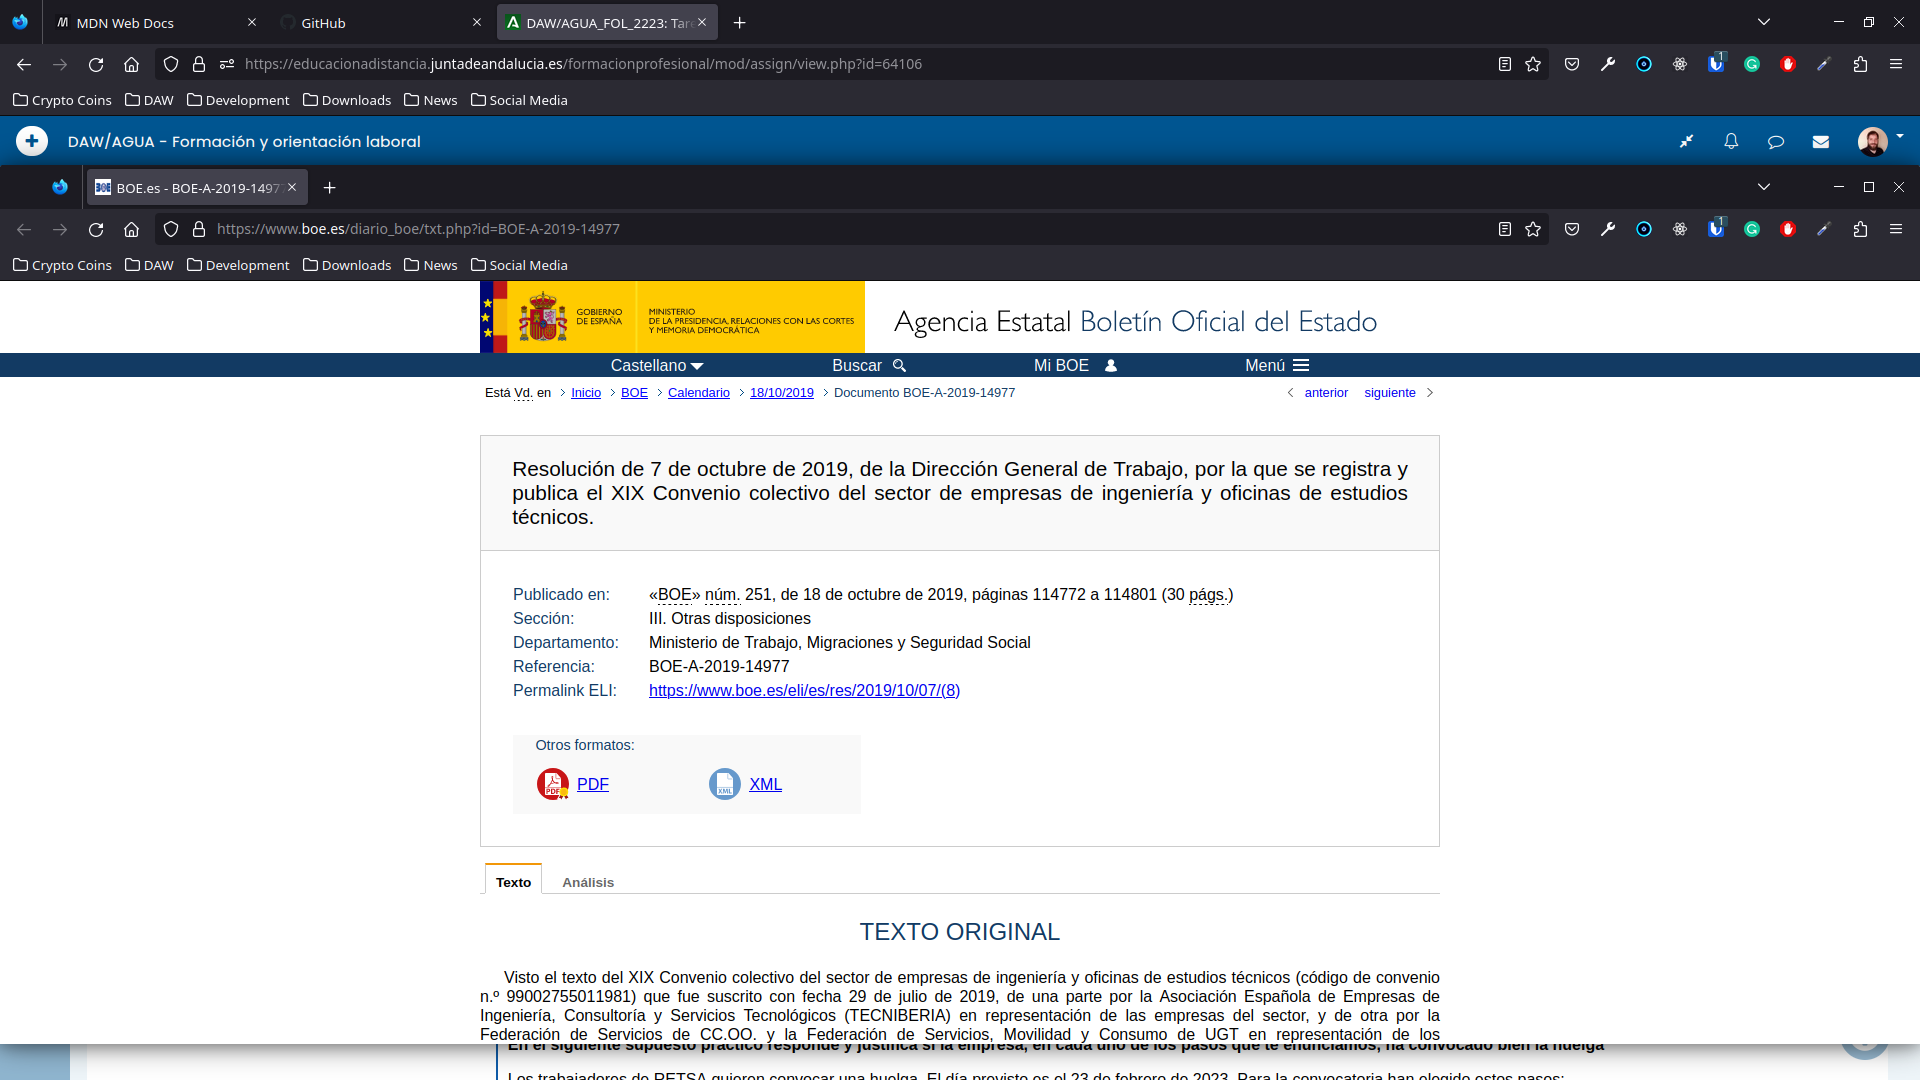
\includegraphics[scale=0.20]{conv-Encabezado.png}
        \caption{Encabezado del convenio colectivo}
    \end{figure}

    \item El contenido mínimo del convenio es el siguiente:
    \begin{enumerate}
        \item El texto, donde se especifican las partes esta en el preámbulo, antes del punto primero, como podemos ver en la siguiente captura:

        \begin{figure}[H]
            \centering
            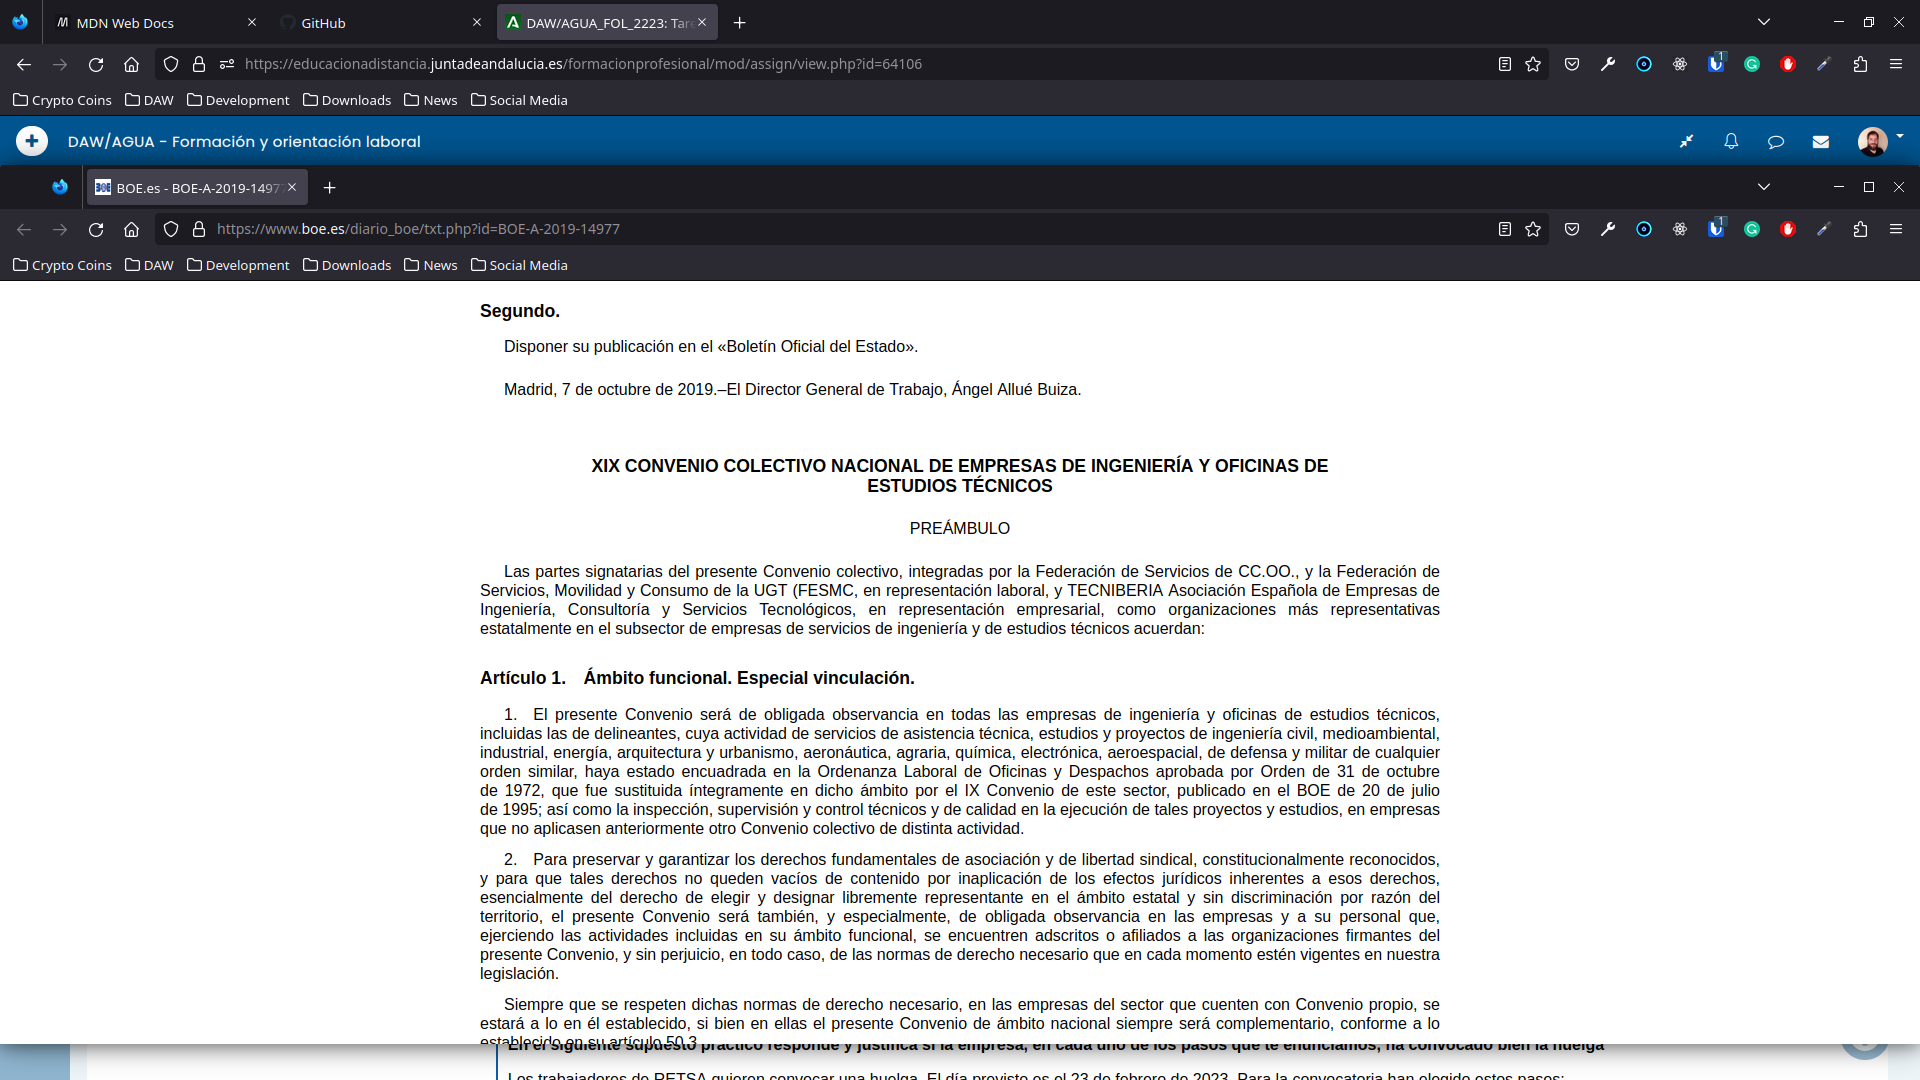
\includegraphics[scale=0.20]{conv-Partes.png}
            \caption{Partes negociadoras en el convenio}
        \end{figure}

        El \textbf{texto} de este punto es el siguiente:

         ``Las partes signatarias del presente Convenio colectivo, integradas por la Federación de Servicios de CC.OO., y la Federación de Servicios, Movilidad y Consumo de la UGT (FESMC, en representación laboral, y TECNIBERIA Asociación Española de Empresas de Ingeniería, Consultoría y Servicios Tecnológicos, en representación empresarial, como organizaciones más representativas estatalmente en el subsector de empresas de servicios de ingeniería y de estudios técnicos acuerdan''

         \item El ámbito de aplicación del convenio, se especifica en los \textbf{artículos 1, 2 3 y 4}, como vemos en la siguiente captura.

          \begin{figure}[H]
             \centering
             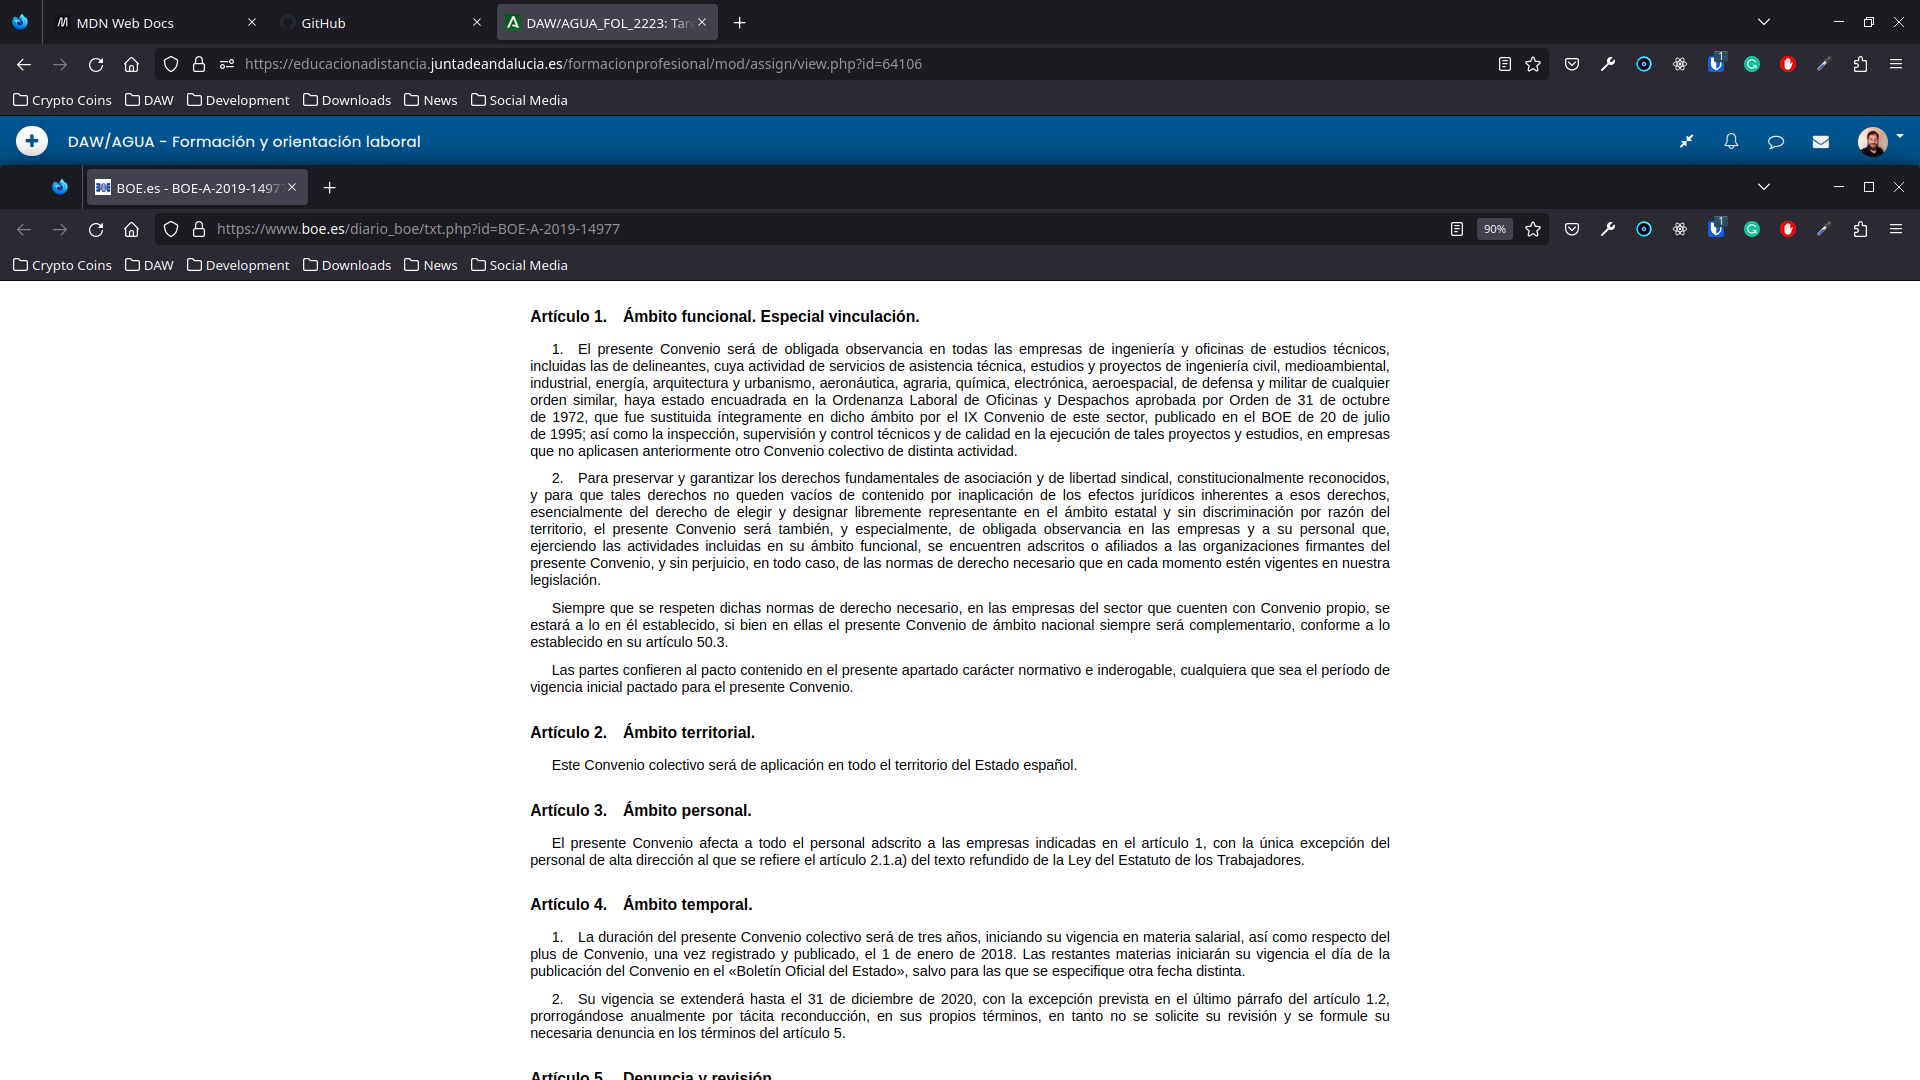
\includegraphics[scale=0.20]{conv-Ambito.png}
             \caption{Ámbito de aplicación del convenio}
         \end{figure}

        Y su \textbf{texto} es el siguiente:

        \begin{itemize}
            \item \textbf{Artículo 1. Ámbito funcional. Especial vinculación.}

            \begin{enumerate}
                \item El presente Convenio será de obligada observancia en todas las empresas de ingeniería y oficinas de estudios técnicos, incluidas las de delineantes, cuya actividad de servicios de asistencia técnica, estudios y proyectos de ingeniería civil, medioambiental, industrial, energía, arquitectura y urbanismo, aeronáutica, agraria, química, electrónica, aeroespacial, de defensa y militar de cualquier orden similar, haya estado encuadrada en la Ordenanza Laboral de Oficinas y Despachos aprobada por Orden de 31 de octubre de 1972, que fue sustituida íntegramente en dicho ámbito por el IX Convenio de este sector, publicado en el BOE de 20 de julio de 1995; así como la inspección, supervisión y control técnicos y de calidad en la ejecución de tales proyectos y estudios, en empresas que no aplicasen anteriormente otro Convenio colectivo de distinta actividad.

                \item Para preservar y garantizar los derechos fundamentales de asociación y de libertad sindical, constitucionalmente reconocidos, y para que tales derechos no queden vacíos de contenido por inaplicación de los efectos jurídicos inherentes a esos derechos, esencialmente del derecho de elegir y designar libremente representante en el ámbito estatal y sin discriminación por razón del territorio, el presente Convenio será también, y especialmente, de obligada observancia en las empresas y a su personal que, ejerciendo las actividades incluidas en su ámbito funcional, se encuentren adscritos o afiliados a las organizaciones firmantes del presente Convenio, y sin perjuicio, en todo caso, de las normas de derecho necesario que en cada momento estén vigentes en nuestra legislación.
            \end{enumerate}

            Siempre que se respeten dichas normas de derecho necesario, en las empresas del sector que cuenten con Convenio propio, se estará a lo en él establecido, si bien en ellas el presente Convenio de ámbito nacional siempre será complementario, conforme a lo establecido en su artículo 50.3.

            Las partes confieren al pacto contenido en el presente apartado carácter normativo e inderogable, cualquiera que sea el período de vigencia inicial pactado para el presente Convenio.

            \item \textbf{Artículo 2. Ámbito territorial.}

            Este Convenio colectivo será de aplicación en todo el territorio del Estado español.

            \item \textbf{Artículo 3. Ámbito personal.}

             El presente Convenio afecta a todo el personal adscrito a las empresas indicadas en el artículo 1, con la única excepción del personal de alta dirección al que se refiere el artículo 2.1.a) del texto refundido de la Ley del Estatuto de los Trabajadores.

             \item \textbf{Artículo 4. Ámbito temporal.}
             \begin{enumerate}
                 \item La duración del presente Convenio colectivo será de tres años, iniciando su vigencia en materia salarial, así como respecto del plus de Convenio, una vez registrado y publicado, el 1 de enero de 2018. Las restantes materias iniciarán su vigencia el día de la publicación del Convenio en el «Boletín Oficial del Estado», salvo para las que se especifique otra fecha distinta.

                 \item En el caso de solicitarse la revisión del Convenio, la parte que formule su denuncia deberá simultáneamente presentar comunicación de la promoción de la negociación con propuesta concreta sobre los puntos, el contenido mínimo que comprenda la revisión solicitada y requisitos establecidos en el artículo 89.1 del Estatuto de los Trabajadores. Caso de incumplimiento, se tendrá por no hecha la denuncia. De esta comunicación y de la propuesta se enviará copia, a efectos de registro, a la Dirección General de Empleo.
             \end{enumerate}
        \end{itemize}
    \end{enumerate}

       \item El texto referente a las vacaciones se encuentra en el \textbf{Articulo 23}, como se muestra en la captura de pantalla.

    \begin{figure}[H]
        \centering
        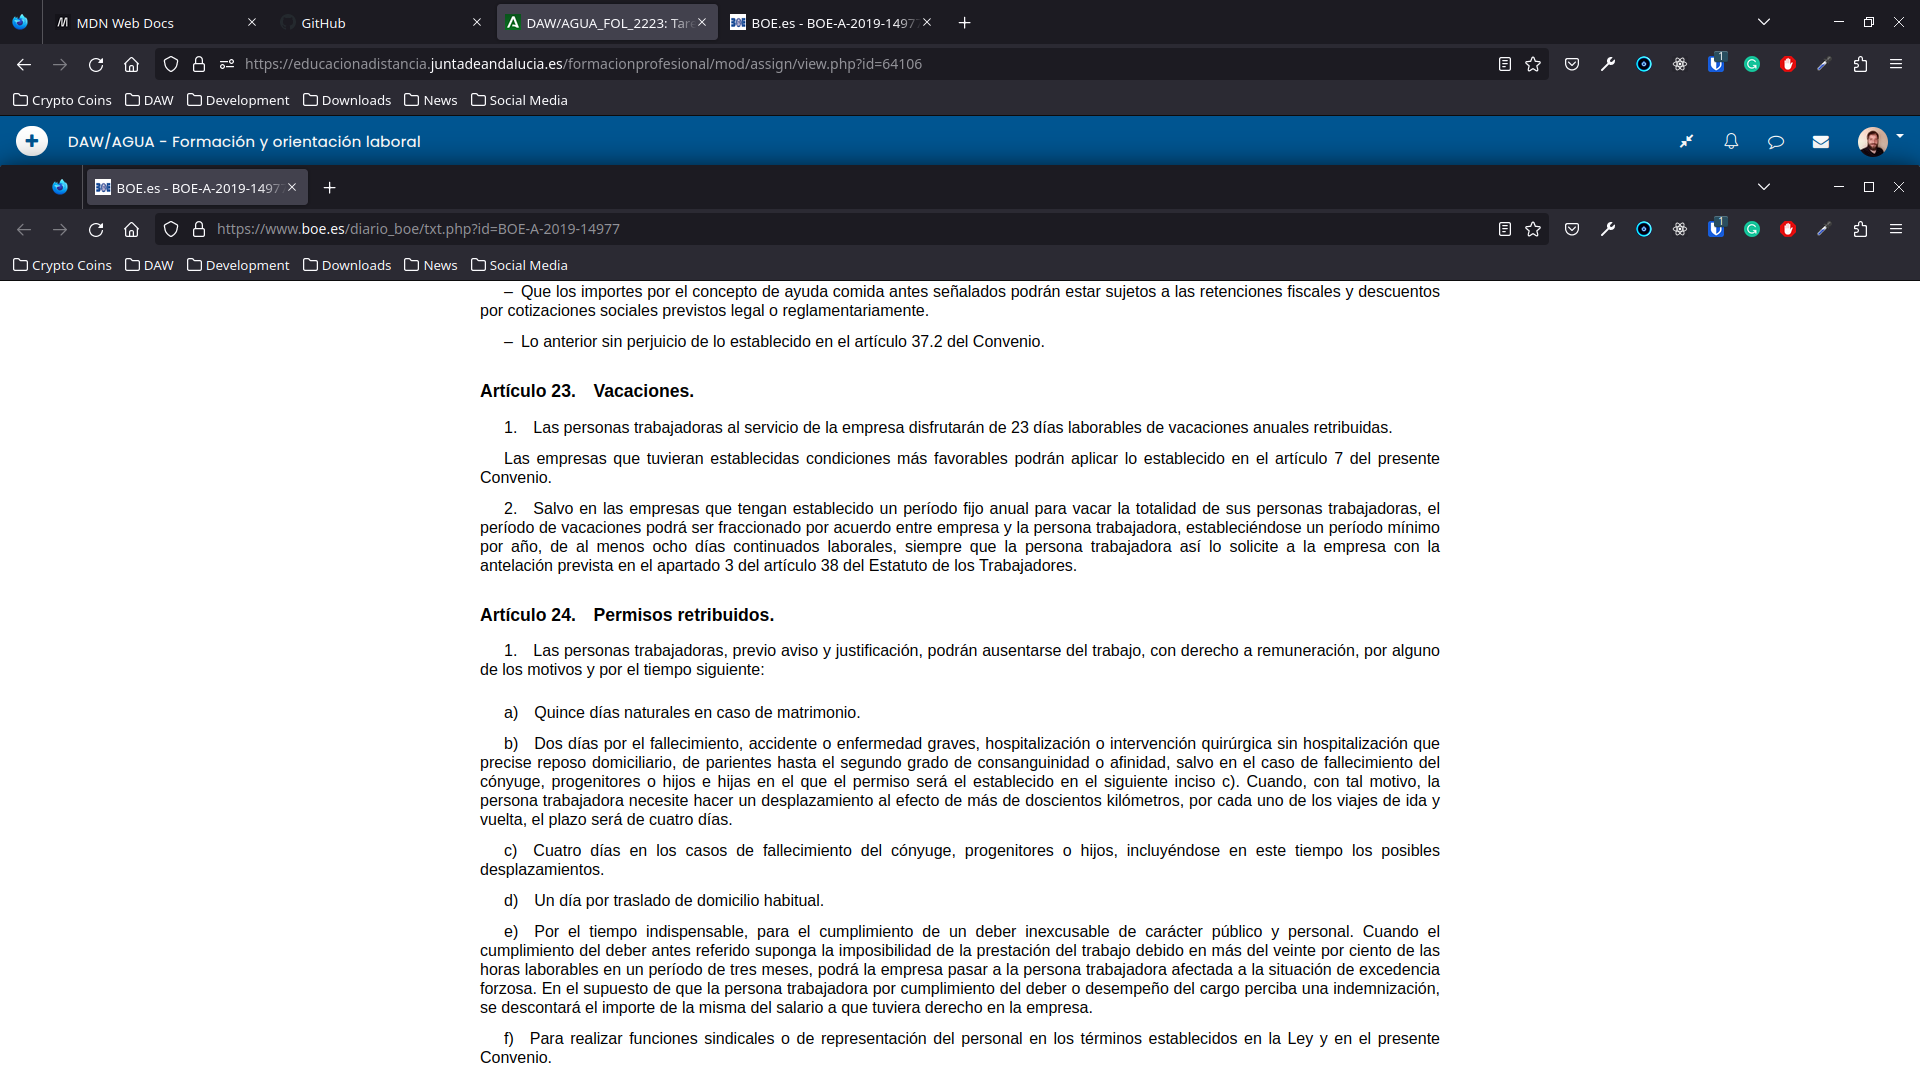
\includegraphics[scale=0.19]{conv-Vaca.png}
        \caption{Normativa sobre las vacaciones en el convenio}
    \end{figure}

    Siendo el \textbf{texto} sobre este tema el siguiente:

    \begin{itemize}
        \item \textbf{Artículo 23. Vacaciones.}
        \begin{enumerate}
            \item Las personas trabajadoras al servicio de la empresa disfrutarán de 23 días laborables de vacaciones anuales retribuidas.

            Las empresas que tuvieran establecidas condiciones más favorables podrán aplicar lo establecido en el artículo 7 del presente Convenio.

            \item Salvo en las empresas que tengan establecido un período fijo anual para vacar la totalidad de sus personas trabajadoras, el período de vacaciones podrá ser fraccionado por acuerdo entre empresa y la persona trabajadora, estableciéndose un período mínimo por año, de al menos ocho días continuados laborales, siempre que la persona trabajadora así lo solicite a la empresa con la antelación prevista en el apartado 3 del artículo 38 del Estatuto de los Trabajadores.
        \end{enumerate}
    \end{itemize}

    \item El artículo elegido es el \textbf{artículo 12. Promociones o Ascensos}, que como su propio nombre indica, trata sobre las promociones en las empresas en las que se aplique este convenio. En la siguiente figura se muestra una captura de este artículo.

    \begin{figure}[ht]
        \centering
        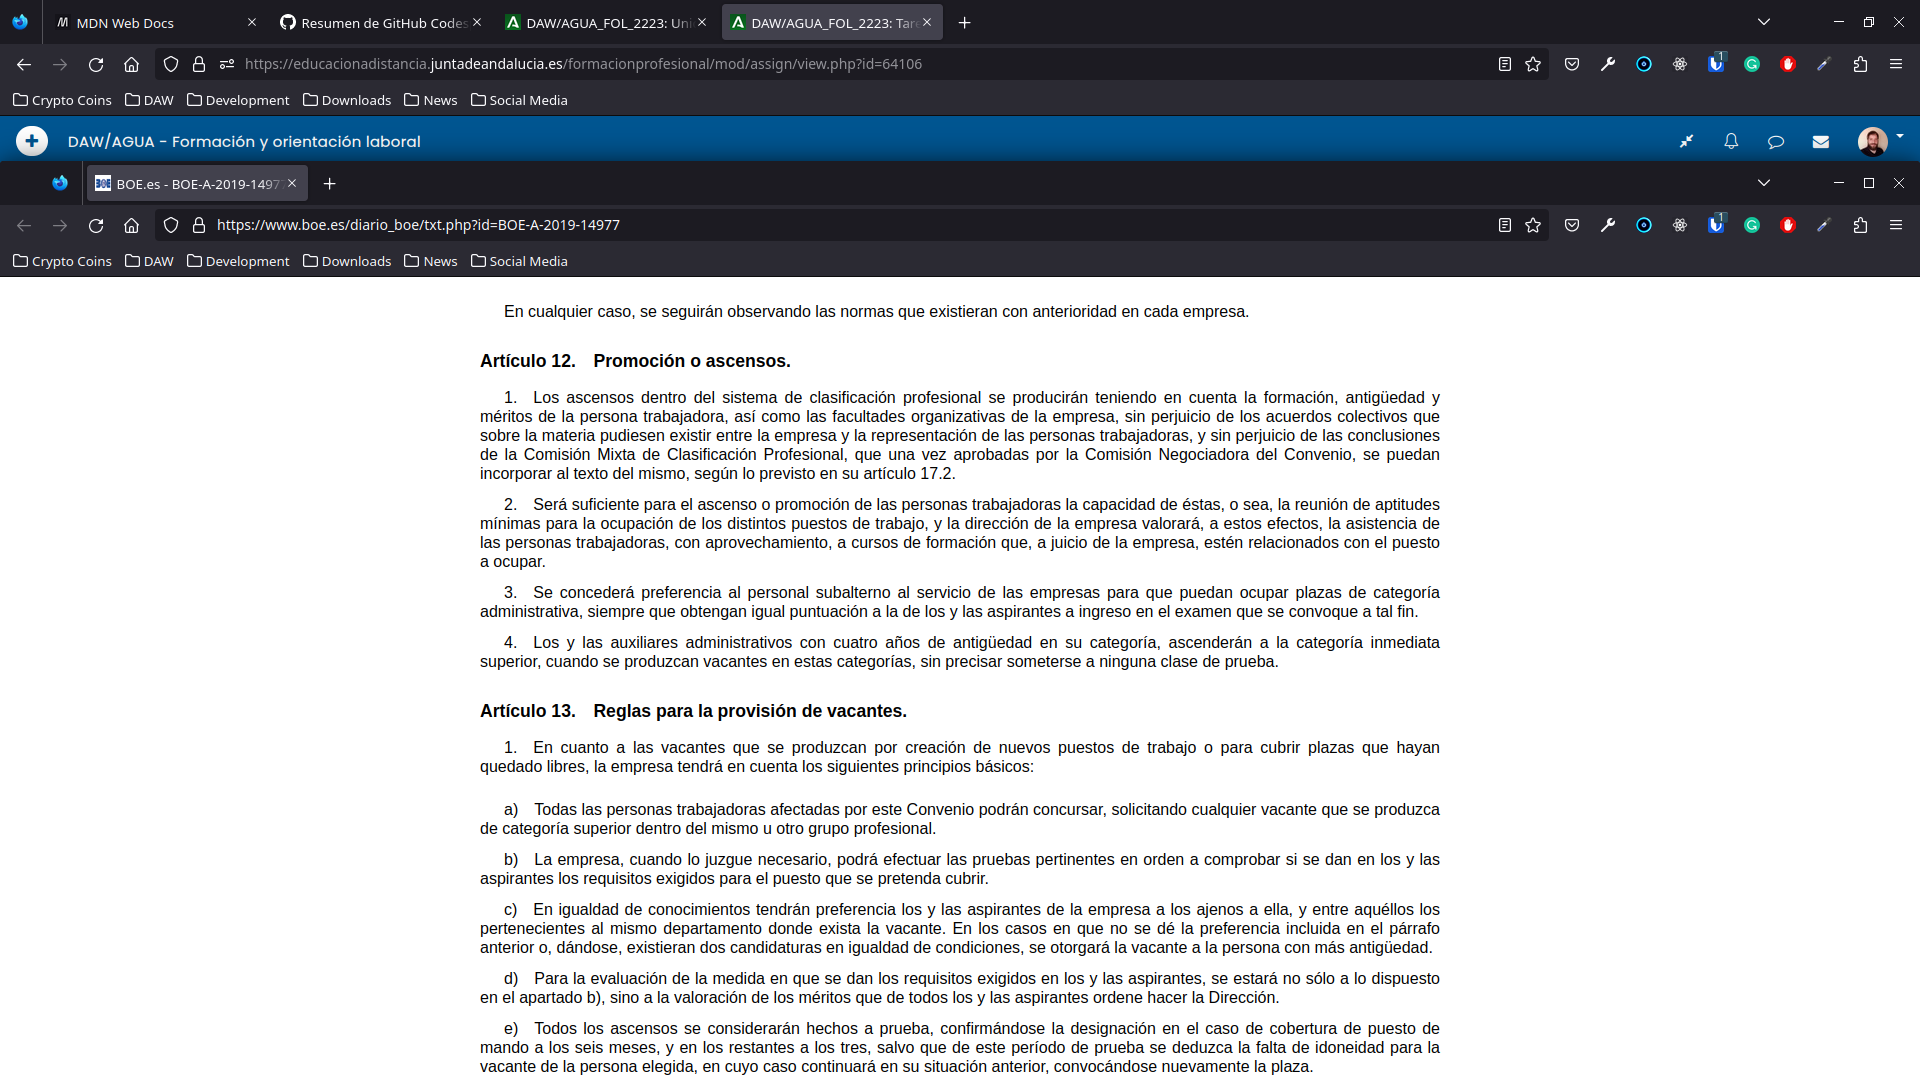
\includegraphics[scale=0.20]{conv-Promo.png}
        \caption{Articulo 12 del convenio}
    \end{figure}

    El \textbf{texto} del artículo reza así:

    \begin{itemize}
        \item \textbf{Artículo 12. Promoción o ascensos.}
        \begin{enumerate}
            \item Los ascensos dentro del sistema de clasificación profesional se producirán teniendo en cuenta la formación, antigüedad y méritos de la persona trabajadora, así como las facultades organizativas de la empresa, sin perjuicio de los acuerdos colectivos que sobre la materia pudiesen existir entre la empresa y la representación de las personas trabajadoras, y sin perjuicio de las conclusiones de la Comisión Mixta de Clasificación Profesional, que una vez aprobadas por la Comisión Negociadora del Convenio, se puedan incorporar al texto del mismo, según lo previsto en su artículo 17.2.

            \item Será suficiente para el ascenso o promoción de las personas trabajadoras la capacidad de éstas, o sea, la reunión de aptitudes mínimas para la ocupación de los distintos puestos de trabajo, y la dirección de la empresa valorará, a estos efectos, la asistencia de las personas trabajadoras, con aprovechamiento, a cursos de formación que, a juicio de la empresa, estén relacionados con el puesto a ocupar.

            \item Se concederá preferencia al personal subalterno al servicio de las empresas para que puedan ocupar plazas de categoría administrativa, siempre que obtengan igual puntuación a la de los y las aspirantes a ingreso en el examen que se convoque a tal fin.

            \item Los y las auxiliares administrativos con cuatro años de antigüedad en su categoría, ascenderán a la categoría inmediata superior, cuando se produzcan vacantes en estas categorías, sin precisar someterse a ninguna clase de prueba.
        \end{enumerate}
    \end{itemize}

    Este artículo me ha \textbf{llamado la atención} porque mientras que en muchos otros sectores lo \textbf{ascensos}, especialmente aquí en España, no están regulados, en el \textbf{sector del desarrollo de software} es algo bastante \textbf{normal}, lo que me parece estupendo ya que es una \textbf{motivación extra} para los \textbf{trabajadores}, el saber que pueden progresar en su carrera profesional.

    El artículo determina que para el ascenso \textbf{será suficiente} con que el trabajador tenga las \textbf{competencias adecuadas} para el desarrollo de la actividad en el \textbf{nuevo puesto}, lo que me parece estupendo, ya que esto motivará a los trabajadores a tener una mentalidad abierta a la formación continua así como a dar el 100\% en su puesto poniendo interés en aprender cosas nuevas y evolucionar.
\end{enumerate}

\section{Actividad 3}

\subsection{Enunciado}

\subsubsection*{Los conflictos colectivos}

\begin{enumerate}
    \item Define qué es un conflicto colectivo.
    \item Cita y diferencia los medios de  resolución extrajudicial de los conflictos colectivos cuando se prevean en los convenios colectivos.
\end{enumerate}

\subsection{Respuesta}
\begin{enumerate}
    \item Un \textbf{conflicto colectivo} es un conflicto que afecta a los intereses generales de los trabajadores, en contraposición a un conflicto individual que solo afectara a los intereses de una trabajador. Podemos encontrar dos tipos de conflictos colectivos:

    \begin{itemize}
        \item \textbf{Conflicto económico o de intereses}: cuando se quiere modificar o sustituir una norma que regular las condiciones de trabaja por otra más beneficiosa.
        \item \textbf{Conflicto jurídico}: cuando no hay acuerdo en la interpretación o aplicación de una normal.
    \end{itemize}

    Cabe destacar, que no podrá plantearse un conflicto colectivo para modificar lo \textbf{pactado en Convenio Colectivo}. \cite{rd1777}

    \item Los \textbf{medios extrajudiciales} para la solución de conflictos establecidos en \textbf{convenios colectivos} constituyen una serie de mecanismos que se resumen en los siguiente:

    \begin{itemize}
        \item \textbf{Mediación}: en este caso, las partes están obligadas a negociar con la ayuda de una o varios personas  que intentarán que se alcance un acuerdo, pudiendo estas personas, llamadas mediadores, hacer propuestas que podrán o no aceptar las partes.

        \item \textbf{Arbitraje}: a diferencia de la mediación, en el arbitraje interviene una tercera parte, denominada \textbf{arbitro} y elegida por ambas partes o impuesto por la administración, que interviene en la negociación de forma activa y su decisión, llamada \textbf{laudo arbitral}, es obligatoria para ambas partes.

        A diferencia de la medición, donde el mediador puede hacer propuestas que las partes pueden aceptar o no, en el arbitraje, las propuestas que haga el arbitro son vinculantes y de obligatoria aceptación por ambas partes.

        \item \textbf{Conciliación}: en este caso, las partes negocian por si solas para llegar a un acuerdo. Un elemento de este tipo de medida que favorece la conciliación son las \textbf{comisiones paritarias} establecidas en los convenios y que median para que se llegue a un acuerdo sin la necesidad de tomar medidas de presión como la convocatoria de una huelga.

        Al contrario que en las dos medidas anteriores, en la conciliación no interviene ninguna parte externa a las partes interesadas para mediar en el conflicto, sino que los únicos intervinientes son las partes interesadas.
    \end{itemize}
\end{enumerate}

\section{Actividad 4}
\subsection{Enunciado}

\subsubsection*{Huelga y Cierre Patronal}
En el siguiente supuesto práctico responde y justifica si la empresa, en cada uno de los pasos que te enunciamos, ha convocado bien la huelga:

Los trabajadores de RETSA quieren convocar una huelga. El día previsto es el 23 de febrero de 2023. Para la convocatoria han elegido estos pasos:

\begin{enumerate}
    \item Realizan una asamblea representativa de los trabajadores afectados, donde exponen la información del problema, deciden las acciones que van a llevar a cabo y las recogen en un acta. A la asamblea acuden 180 trabajadores de los 300 que hay en la plantilla. Los votos a favor de la huelga han sido 91, en contra 81  y 8 abstenciones.
    \item Tienen previsto entregar el documento de información de la convocatoria de huelga en la Dirección General de Trabajo el día 18 de febrero de 2023, adjuntando la copia del acta de la asamblea, las hojas de asistencias y el documento de los eventos realizados para evitar la huelga.
    \item Constituyen un comité de huelga formado por 13 personas.
\end{enumerate}

Además,

\begin{enumerate}[label=(\alph*)]
    \item Comenta todas y cada una de las consecuencias que tiene para el trabajador el llevar a cabo una huelga legalmente convocada.
    \item Explica brevemente sobre los servicios mínimos:
    \begin{enumerate}
        \item ¿Qué son?
        \item ¿Cuándo se decretan.
        \item ¿Quién/es lo determinan?
        \item Pon un ejemplo.
    \end{enumerate}
\end{enumerate}

\subsection{Respuesta}

\begin{enumerate}
    \item Este primer punto si \textbf{se ha llevado a cabo de forma correcta}. Se ha creado un asamblea representativa, donde han acudido más de un 25\% de los trabajadores afectados, como estipula el Real Decreto-ley 1977/17, se ha decidido declarar una huelga con un resultado de la votación a favor por mayoría simple, además, se han recogido en acta todas las decisiones que se han tomado y las acciones que se van a llevar a cabo.

    \item Este punto \textbf{no se ha realizado correctamente}, ya que aunque se le ha notificado con la documentación adecuada la convocatoria de huelga a la Dirección General de Trabajo, y ademas, se ha hecho con más de 5 días de antelación, no se ha notificado a la empresa, lo que es obligatorio segun el RD 1977/17.

    \item Este punto \textbf{tampoco se ha llevado a cabo correctamente}, ya que el número máximo de miembros del comité de huelga es de 12, y los trabajadores han creado un comité
\end{enumerate}

\begin{enumerate}[label=(\alph*)]
    \item Cuando un trabajador lleva a cabo un huelga, las consecuencias son las siguientes:
    \begin{enumerate}
        \item \textbf{Reserva del puesto de trabajo}: durante la huelga se suspende el contrato de trabajo, retomándose una vez finalizada esta y sin que los días de huelga afecten a los días de absentismo o a las vacaciones.

        \item \textbf{Cese del pago del salario}: al suspenderse el contrato de trabajo el trabajador no estará obligado a acudir a su puesto de trabajo, pero el empresario tampoco estará obligado a pagarle su salario durante esos días.

        \item \textbf{Seguridad Social}: durante los días de huelga se suspende también la cotización del trabajador en la Seguridad Social, tanto para la empresa como para el trabajador, quién quedará en situación de \textit{alta especial}.

        \item \textbf{Responsabilidad disciplinaria}: nadie puede ser despedido o sancionado por ejercer su derecho a huelga siempre que esta sea legal.

        \item \textbf{Sustituciones}: está prohibido que el empresario pueda contratar a otros trabajadores para ocupar los puestos de los huelguistas, lo que se conoce como \textbf{esquirolaje}.
    \end{enumerate}
    \item Explica brevemente sobre los servicios mínimos:
    \begin{enumerate}
        \item Los \textbf{servicios mínimos} son aquellos servicios que se consideran esenciales y que se siguen prestando durante una huelga para garantizar que no haya desabastecimiento, caos, falta de producción, etc.. \cite{wiki01}. Son, de hecho, una limitación del derecho a huelga.

        \item Los servicios mínimos se deben decretar antes del día de la huelga, para poder informar a los trabajadores que deberán acudir a sus puestos de trabajo para garantizar estos servicios mínimos.

        \item Los servicios mínimos los determina la \textbf{autoridad gubernamental competente}. Dependiendo de a que sector afecte, será algún ministerio, u otras autoridades gubernamentales ya sean autonómicas o nacionales, dependiendo también del alcance de la huelga.

        Por ejemplo, si es una huelga que afecta a los transportes públicos a nivel nacional, será el \textbf{Ministerio de Transportes} el encargado de establecer los servicios mínimos.

        \item Un ejemplo reciente ha sido la huelga convocada por el \textbf{Sindicato Autónomo de Trabajadores de Empresas de Seguridad}, que ha afectado al aeropuerto Aeropuerto Adolfo Suárez Madrid-Barajas, que comenzó el día 22 de Diciembre.

        En este caso, el \textbf{Ministerio de Transportes, Movilidad y Agenda Urbana} decretó una serie de servicios esenciales, el día 21 de Diciembre, para garantizar la seguridad en dicho aeropuerto, en concreto, para los \textbf{servicios de seguridad en filtros}.

        En el siguiente  \href{https://www.mitma.gob.es/recursos_mfom/paginabasica/recursos/resolucion_ssmm_huelga_servicios_auxiliares_de_seguridad_sagital.pdf}{este enlace} podemos encontrar el documento con la resolución de los servicios mínimos decretados.
    \end{enumerate}
\end{enumerate}

\section{Actividad 5}
\subsection{Enunciado}

\subsubsection*{Huelga y Cierre Patronal}
\begin{enumerate}
    \item Aconseja a la empresa sobre la siguiente situación que se plantea:

    ``Durante una huelga legalmente convocada la empresa, harta de la situación, se plantea dos opciones. La primera es despedir a los dos trabajadores que tiene trabajando y  que van a secundar la huelga. La segunda, sustituir a esos dos trabajadores durante el tiempo que dure''

    \item Comenta las consecuencias que tiene para la persona trabajadora el cierre legal de su empresa.

    \item Busca una noticia en los medios de comunicación sobre una huelga o cierre patronal durante este año 2022, publícala en el foro, sube la captura del foro a la tarea y además haz un análisis en relación al contenido tratado en el tema. Si la noticia ya está subida por algún compañer@ (no se pueden repetir), puedes optar por hacer un comentario en el que se manifieste tu valoración personal sobre ella en el foro, captura tal aportación y la adjuntas a la tarea junto con un análisis en el que has de trabajar el contenido tratado en el tema en relación a la noticia.
\end{enumerate}

\subsection{Respuesta}

\begin{enumerate}
    \item Mi recomendación sería que no realizara ninguna de esas acciones, ya que son ilegales y podría verse en problemas. Un cierre patronal tampoco tendría sentido, porque a fin de cuentas, la situación sería parecida a la que se esta viviendo por la huelga, por lo que le recomendaría que ejerciera otras medidas de presión como:

    \begin{itemize}
        \item Circulación de "listas negras" de los trabajadores que tengan una actitud reivindicativa.
        \item Transmisión de información entre empresas acerca del comportamiento sindical de los trabajadores.
        \item Despidos colectivos en situaciones de conflictos.
    \end{itemize}

    \item Las \textbf{consecuencias} de un cierre patronal para un trabajador son similares a las de una huelga:
    \begin{itemize}
        \item Prohibición de acceder al puesto de trabajo.
        \item Perdida del derecho a percibir su salario.
        \item El contrato queda suspendido, a los mismos efectos que en una huelga.
        \item Se suspende la obligación de cotización y este quedaría en alta especial.
        \item Perdida de derecho a percibir prestaciones por incapacidad o desempleo durante el cierre patronal.
    \end{itemize}

    \item En este caso he elegido una noticia sobre la huelga de los \textbf{trabajadores} de la \textbf{planta de Trapagarán de Amazon}, que se llevo a cabo el \textbf{17 de Octubre de 2022}.

    Los \textbf{convocantes} de la huelga son los \textbf{109 trabajadores} de la planta y el \textbf{sindicato LAB}, que tiene mayoría en el comité. La huelga tuvo una duración de \textbf{4 horas} durante el día 17 de Octubre, entre las 5:30 y las 9:30 h y la principales reivindicaciones de los trabajadores son, entre otras, las siguientes:

    \begin{itemize}
        \item Elaboración de un convenio colectivo, ya que actualmente se rigen por el convenio de transportistas de Euskadi.
        \item Actualización de los salarios con el IPC.
        \item Derecho a la subrogación de los repartidores de paquetes.
    \end{itemize}

     \begin{figure}[H]
        \centering
        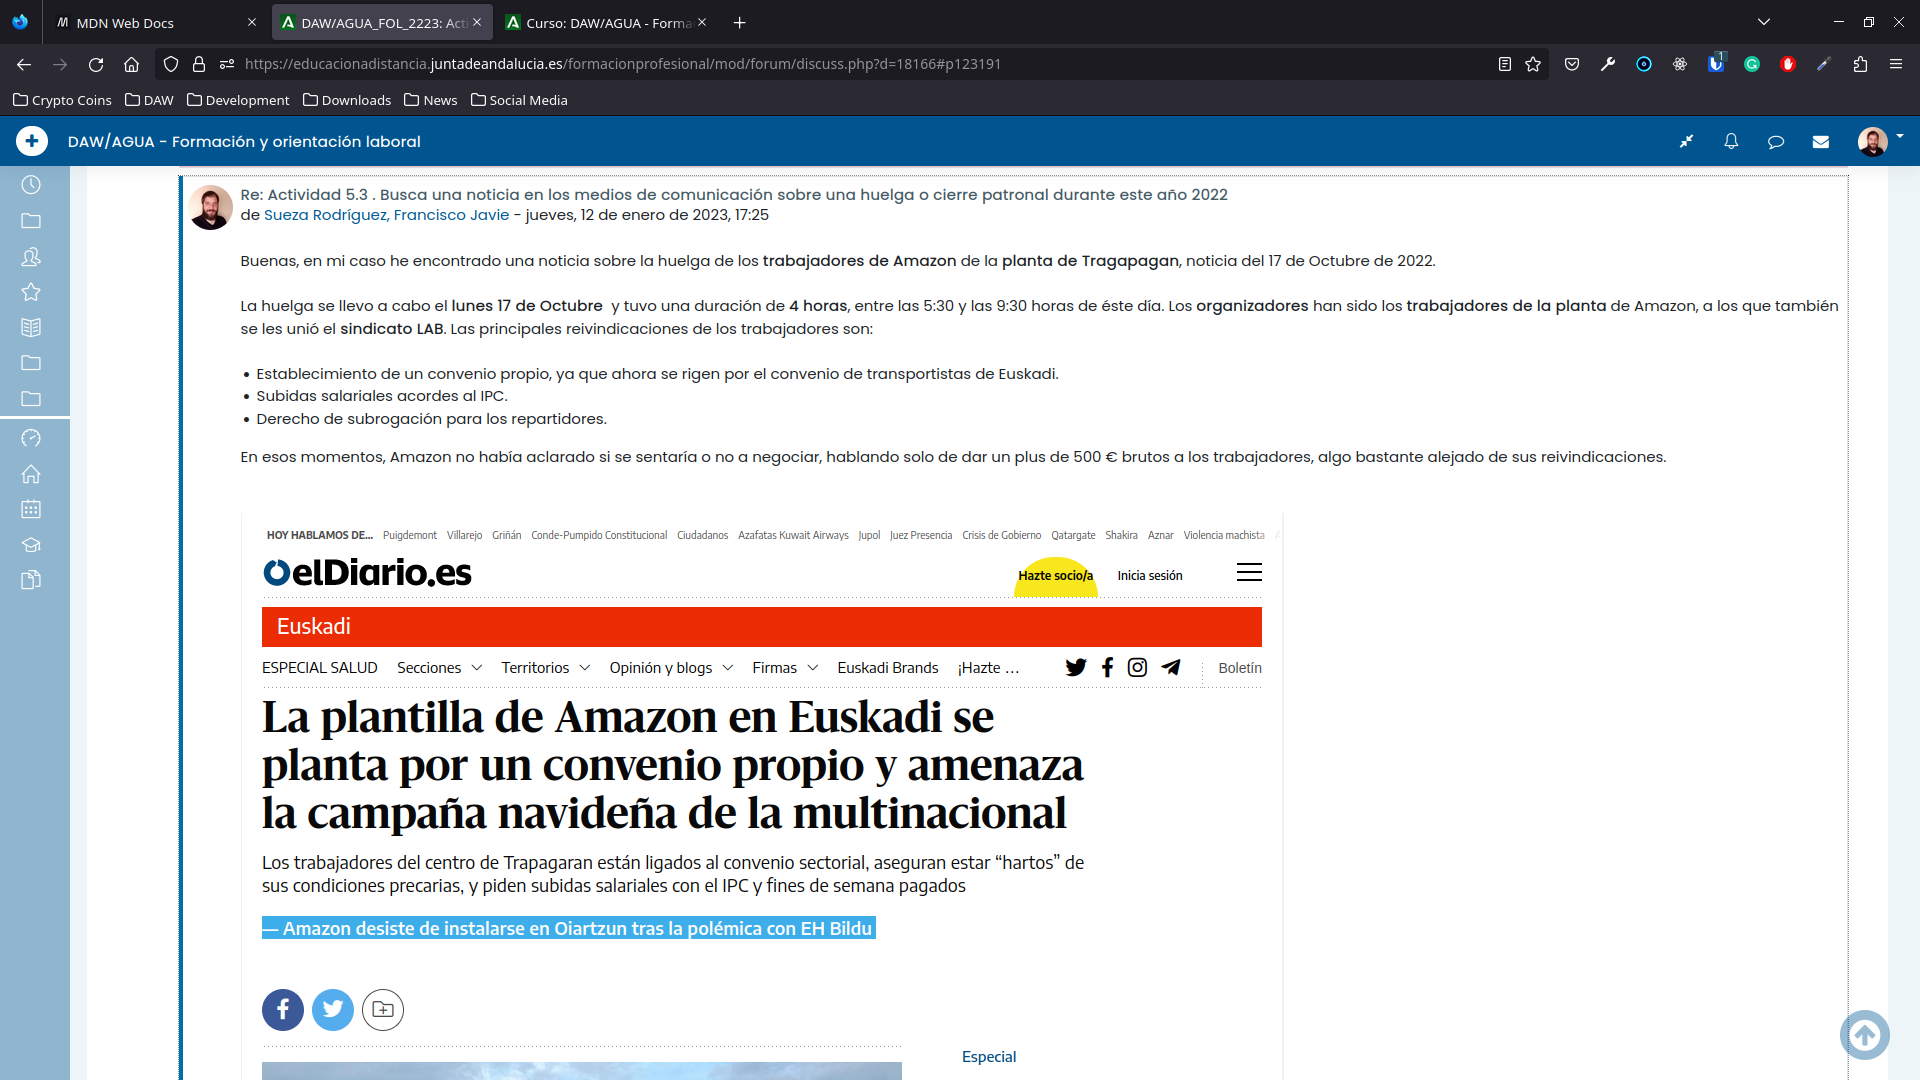
\includegraphics[scale=0.20]{screen-foro.png}
        \caption{Imagen del mensaje en el foro}
    \end{figure}

    En la noticia no menciona si antes de llegar a esta situación se ha intentado llegar a un acuerdo usando algunos de los procedimientos pacíficos para su solución, aunque según los comentarios de los representantes de Amazon, no parece que la empresa tenga intención, por el momento, de acceder a las exigencias de los trabajadores.

    Al parecer, y según podemos ver en \href{https://www.eldiario.es/euskadi/exito-huelga-amazon-bizkaia-60-000-paquetes-bloqueados-puertas-navidad_1_9820882.html}{noticias más recientes}, el conflicto sigue sin solucionarse, por lo que la empresa no se ha sentado aun con los trabajadores, o sí lo ha hecho, no ha sido para acceder a sus demandas.
\end{enumerate}









% Bibliography

\newpage
\bibliography{citas}
\bibliographystyle{unsrt}

\end{document}